\documentclass[11pt]{article}
\usepackage[utf8]{inputenc}
\usepackage{a4wide}
\usepackage{graphicx}

% Sources :
% 1) https://gist.github.com/chi-feng/6589066/4cda665ff0d93b8611a0e047a6a06d6a8ecd9b4e
% 2) https://groups.google.com/forum/#!topic/julia-dev/HHjlYalHXY8

\usepackage{inconsolata} % very nice fixed-width font included with texlive-full
\usepackage[usenames,dvipsnames]{color} % more flexible names for syntax highlighting colors
\usepackage{listings}

\lstset{
basicstyle=\ttfamily, 
columns=fullflexible, % make sure to use fixed-width font, CM typewriter is NOT fixed width
numbers=left, 
numberstyle=\small\ttfamily\color{Gray},
stepnumber=1,              
numbersep=10pt, 
numberfirstline=true, 
numberblanklines=true, 
tabsize=4,
lineskip=-1.5pt,
extendedchars=true,
breaklines=true,        
keywordstyle=\color{Blue}\bfseries,
identifierstyle=, % using emph or index keywords
commentstyle=\sffamily\color{OliveGreen},
stringstyle=\color{Maroon},
showstringspaces=false,
showtabs=false,
upquote=false,
texcl=true % interpet comments as LaTeX
}

\lstdefinelanguage{julia}
{
  keywordsprefix=\@,
  morekeywords={
    exit,whos,edit,load,is,isa,isequal,typeof,tuple,ntuple,uid,hash,finalizer,convert,promote,
    subtype,typemin,typemax,realmin,realmax,sizeof,eps,promote_type,method_exists,applicable,
    invoke,dlopen,dlsym,system,error,throw,assert,new,Inf,Nan,pi,im,begin,while,for,in,return,
    break,continue,macro,quote,let,if,elseif,else,try,catch,end,bitstype,ccall,do,using,module,
    import,export,importall,baremodule,immutable,local,global,const,Bool,Int,Int8,Int16,Int32,
    Int64,Uint,Uint8,Uint16,Uint32,Uint64,Float32,Float64,Complex64,Complex128,Any,Nothing,None,
    function,type,typealias,abstract
  },
  sensitive=true,
  morecomment=[l]{\#},
%  morecomment=[s]{# =}{=#},
  morestring=[b]',
  morestring=[b]" 
}

\title{Examples of using \\ vOptSpecific, vOptGeneric, and vOptTools}
\author{Xavier Gandibleux }
\date{\today}

\begin{document}
\maketitle
\abstract{This document provides examples of using vOptSpecific, vOptGeneric, and vOptTools.}
\vspace{5mm}

\tableofcontents
\break

%
% ==========================================================================================
%
\section{Examples with the bi-objective linear assignment problem}

\vspace{5mm} \noindent {\large  \textbf{The bi-objective linear assignment problem (2LAP)}} \vspace{5mm} 

$$
\quad
\left [
\begin{array}{cllllll}

  \min z^k&  =  & \displaystyle{\sum_{i=1}^{n}\sum_{j=1}^{n} c^k_{ij} x_{ij}}  &  k=1,\dots,2\vspace{2mm} \\

  s/c &\  &   \displaystyle{\sum_{i=1}^{n}  x_{ij}}   =  1 &   j=1,\dots ,n \  \ \  \\
        &  &   \displaystyle{\sum_{j=1}^{n}  x_{ij}}   =  1 &  i=1,\dots ,n \    \vspace{2mm} \\

&  &   x_{ij} = (0,1) &   i=1,\dots ,n  \vspace{-1mm}\\
&  &    &  j=1,\dots ,n\\ 
 
\end{array}
\right ]
$$

\vspace{5mm} \noindent {\large  \textbf{A numerical instance of 2LAP}} \vspace{5mm} 


%\begin{verbatim}
$$
C^1 = \left(\begin{array}{ccccc}
3  & 9 &  7 \\
16 &  10  & 6  \\
2  & 7 & 11    
\end{array}
\right)
$$
\medskip

$$
C^2 = \left(\begin{array}{ccccc}
16 &  15 &  6  \\
5 &  7 & 13   \\
1 &  2 & 13 
\end{array}
\right)
$$


\break

\lstset{literate=
  {α}{{$\alpha$}}1 {Δ}{{$\Delta$}}1
  {á}{{\'a}}1 {é}{{\'e}}1 {í}{{\'i}}1 {ó}{{\'o}}1 {ú}{{\'u}}1
  {Á}{{\'A}}1 {É}{{\'E}}1 {Í}{{\'I}}1 {Ó}{{\'O}}1 {Ú}{{\'U}}1
  {à}{{\`a}}1 {è}{{\`e}}1 {ì}{{\`i}}1 {ò}{{\`o}}1 {ù}{{\`u}}1
  {À}{{\`A}}1 {È}{{\'E}}1 {Ì}{{\`I}}1 {Ò}{{\`O}}1 {Ù}{{\`U}}1
  {ä}{{\"a}}1 {ë}{{\"e}}1 {ï}{{\"i}}1 {ö}{{\"o}}1 {ü}{{\"u}}1
  {Ä}{{\"A}}1 {Ë}{{\"E}}1 {Ï}{{\"I}}1 {Ö}{{\"O}}1 {Ü}{{\"U}}1
  {â}{{\^a}}1 {ê}{{\^e}}1 {î}{{\^i}}1 {ô}{{\^o}}1 {û}{{\^u}}1
  {Â}{{\^A}}1 {Ê}{{\^E}}1 {Î}{{\^I}}1 {Ô}{{\^O}}1 {Û}{{\^U}}1
  {œ}{{\oe}}1 {Œ}{{\OE}}1 {æ}{{\ae}}1 {Æ}{{\AE}}1 {ß}{{\ss}}1
  {ű}{{\H{u}}}1 {Ű}{{\H{U}}}1 {ő}{{\H{o}}}1 {Ő}{{\H{O}}}1
  {ç}{{\c c}}1 {Ç}{{\c C}}1 {ø}{{\o}}1 {å}{{\r a}}1 {Å}{{\r A}}1
  {€}{{\EUR}}1 {£}{{\pounds}}1
}


\lstset{language=julia}

%
% ==========================================================================================
%
\subsection{vOptSpecific and 2LAP:\\ data are explicitely provided}

\vspace{5mm} \noindent {\large  \textbf{The program}} \vspace{2mm} \hrule

{%\small
\begin{lstlisting}
n  =  3

C1 = [  3   9   7       ;
       16   10   6     ;
        2      7  11        ]

C2 = [ 16   15   6     ;
         5         7  13     ;
         1         2  13          ]

using vOptSpecific   

m = set2LAP( n , C1 , C2 )
z1, z2, S = vSolve( m )    # solver by default: LAP\_Przybylski2008( ) 
\end{lstlisting}
}
\vspace{5mm} \noindent {\large  \textbf{The result}} \vspace{2mm} \hrule

\begin{verbatim}
julia> z1
4-element Array{Int64,1}:
 16
 19
 30
 17

julia> z2
4-element Array{Int64,1}:
 31
 14
 13
 29

julia> S
4x3 Array{Int64,2}:
 0  2  1
 2  1  0
 1  2  0
 2  0  1
\end{verbatim}

\break

%
% ==========================================================================================
%
\subsection{vOptSpecific and 2LAP:\\ data and solver are explicitely provided}

\vspace{5mm} \noindent {\large  \textbf{The program}} \vspace{2mm} \hrule

{%\small
\begin{lstlisting}
n  =  3

C1 = [  3   9   7       ;
       16   10   6     ;
        2      7  11        ]

C2 = [ 16   15   6     ;
         5         7  13     ;
         1         2  13          ]

using vOptSpecific   

m = set2LAP( n , C1 , C2 )
solver = LAP_Przybylski2008( ) 
z1, z2, S = vSolve( m , solver ) 
\end{lstlisting}
}
\vspace{5mm} \noindent {\large  \textbf{The result}} \vspace{2mm} \hrule

\begin{verbatim}
julia> z1
4-element Array{Int64,1}:
 16
 19
 30
 17

julia> z2
4-element Array{Int64,1}:
 31
 14
 13
 29

julia> S
4x3 Array{Int64,2}:
 0  2  1
 2  1  0
 1  2  0
 2  0  1
\end{verbatim}

\break

%
% ==========================================================================================
%
\subsection{vOptSpecific and 2LAP:\\ read data  on a file according to the LAP format}

\vspace{5mm} \noindent {\large  \textbf{The program}} \vspace{2mm} \hrule

{%\small
\begin{lstlisting}
using vOptSpecific   

m = load2LAP("2ap03.dat")
z1, z2, S = vSolve( m )     # solver by default: LAP\_Przybylski2008( ) 
\end{lstlisting}
}


\vspace{5mm} \noindent {\large  \textbf{Example of a datafile (\texttt{2ap03.dat})}} \vspace{2mm} \hrule
\begin{verbatim}
3
 3   9   7       
16  10   6     
 2   7  11        
16  15   6     
 5   7  13     
 1   2  13 
\end{verbatim}

\vspace{5mm} \noindent {\large  \textbf{The result}} \vspace{2mm} \hrule

\begin{verbatim}
julia> z1
4-element Array{Int64,1}:
 16
 19
 30
 17

julia> z2
4-element Array{Int64,1}:
 31
 14
 13
 29

julia> S
4x3 Array{Int64,2}:
 0  2  1
 2  1  0
 1  2  0
 2  0  1
\end{verbatim}
\break

%
% ==========================================================================================
%
\subsection{vOptGeneric and 2LAP (2IP):\\ data are explicitely provided}

\vspace{5mm} \noindent {\large  \textbf{The program}} \vspace{2mm} \hrule

{%\small
\begin{lstlisting}
n  =  3

C1 = [  3   9   7       ;
       16   10   6     ;
        2   7  11        ]

C2 = [ 16   15   6     ;
         5   7  13     ;
         1   2  13          ]
       
using vOptGeneric
using GLPK ; using GLPKMathProgInterface

m = vModel( solver = GLPKSolverMIP() )
@variable( m , x[1:n,1:n] , Bin )
@addobjective( m , Min, sum( C1[i,j]*x[i,j] for i=1:n,j=1:n ) )
@addobjective( m , Min, sum( C2[i,j]*x[i,j] for i=1:n,j=1:n ) )
@constraint( m , cols[i=1:n], sum(x[i,j] for j=1:n) == 1 )
@constraint( m , rows[j=1:n], sum(x[i,j] for i=1:n) == 1 )
solve( m , method = :epsilon , step = 0.5 )
\end{lstlisting}
}

\vspace{5mm} \noindent {\large  \textbf{The result}} \vspace{2mm} \hrule

\begin{verbatim}
julia> print_X_E(m)
(16.0, 31.0) : x[1,1]=1 x[2,3]=1 x[3,2]=1 
(17.0, 29.0) : x[1,2]=1 x[2,3]=1 x[3,1]=1 
(19.0, 14.0) : x[1,3]=1 x[2,2]=1 x[3,1]=1 
(30.0, 13.0) : x[1,3]=1 x[2,1]=1 x[3,2]=1

julia> getY_N(m)
4-element Array{Tuple{Vararg{Float64,N}} where N,1}:
 (16.0, 31.0)
 (17.0, 29.0)
 (19.0, 14.0)
 (30.0, 13.0)
\end{verbatim}
\break
%
% ==========================================================================================
%
\subsection{vOptGeneric and 2LAP (2LP):\\ data are explicitely provided}

\vspace{5mm} \noindent {\large  \textbf{The program}} \vspace{2mm} \hrule

{%\small
\begin{lstlisting}
n  =  3

C1 = [  3   9   7       ;
       16   10   6     ;
        2   7  11        ]

C2 = [ 16   15   6     ;
         5   7  13     ;
         1   2  13          ]
       
using vOptGeneric
using GLPK ; using GLPKMathProgInterface

m = vModel( solver = GLPKSolverLP() )
@variable( m , x[1:n,1:n] >= 0 )
@addobjective( m , Min, sum( C1[i,j]*x[i,j] for i=1:n,j=1:n ) )
@addobjective( m , Min, sum( C2[i,j]*x[i,j] for i=1:n,j=1:n ) )
@constraint( m , cols[i=1:n], sum(x[i,j] for j=1:n) == 1 )
@constraint( m , rows[j=1:n], sum(x[i,j] for i=1:n) == 1 )
solve( m , method = :epsilon , step = 0.5 )
\end{lstlisting}
}

\vspace{5mm} \noindent {\large  \textbf{The result}} \vspace{2mm} \hrule

\begin{verbatim}
julia> getY_N(m)
37-element Array{Tuple{Vararg{Float64,N}} where N,1}:
 (16.0, 31.0)   
 (16.0882, 30.5)
 (16.1765, 30.0)
 (16.2647, 29.5)
 (16.3529, 29.0)
 (16.4412, 28.5)
 (16.5294, 28.0)
 (16.6176, 27.5)
 (16.7059, 27.0)
 (16.7941, 26.5)
 ...              
 (18.4706, 17.0)
 (18.5588, 16.5)
 (18.6471, 16.0)
 (18.7353, 15.5)
 (18.8235, 15.0)
 (18.9118, 14.5)
 (19.0, 14.0)   
 (24.5, 13.5)   
 (30.0, 13.0) 
\end{verbatim}
\break

%
% ==========================================================================================
%
\subsection{vOptGeneric and 2LAP (2IP):\\ write on a file according to the MOP format}

\vspace{5mm} \noindent {\large  \textbf{The program}} \vspace{2mm} \hrule

{%\small
\begin{lstlisting}
n  =  3

C1 = [  3   9   7       ;
       16   10   6     ;
        2   7  11        ]

C2 = [ 16   15   6     ;
         5   7  13     ;
         1   2  13          ]
       
using vOptGeneric
using GLPK ; using GLPKMathProgInterface

m = vModel( solver = GLPKSolverMIP() )
@variable( m , x[1:n,1:n] , Bin )
@addobjective( m , Min, sum( C1[i,j]*x[i,j] for i=1:n,j=1:n ) )
@addobjective( m , Min, sum( C2[i,j]*x[i,j] for i=1:n,j=1:n ) )
@constraint( m , cols[i=1:n], sum(x[i,j] for j=1:n) == 1 )
@constraint( m , rows[j=1:n], sum(x[i,j] for i=1:n) == 1 )
writeMOP( m , "2ap03.mop" )
\end{lstlisting}
}

\vspace{5mm} \noindent {\large  \textbf{Example of a datafile (\texttt{2ap03.mop})}} \vspace{2mm} \hrule

\begin{verbatim}
NAME   vOptModel
OBJSENSE
 MIN
ROWS
 N  OBJ1
 N  OBJ2
 E  CON1
 E  CON2
 E  CON3
 E  CON4
 E  CON5
 E  CON6
COLUMNS
    MARKER    'MARKER'                 'INTORG'
    x_1_1  CON1  1
    x_1_1  CON4  1
    x_1_1  OBJ1  3
    x_1_1  OBJ2  16
    x_1_2  CON1  1
    x_1_2  CON5  1
    x_1_2  OBJ1  9
    x_1_2  OBJ2  15
    x_1_3  CON1  1
    x_1_3  CON6  1
    x_1_3  OBJ1  7
    x_1_3  OBJ2  6
    x_2_1  CON2  1
    x_2_1  CON4  1
    x_2_1  OBJ1  16
    x_2_1  OBJ2  5
    x_2_2  CON2  1
    x_2_2  CON5  1
    x_2_2  OBJ1  10
    x_2_2  OBJ2  7
    x_2_3  CON2  1
    x_2_3  CON6  1
    x_2_3  OBJ1  6
    x_2_3  OBJ2  13
    x_3_1  CON3  1
    x_3_1  CON4  1
    x_3_1  OBJ1  2
    x_3_1  OBJ2  1
    x_3_2  CON3  1
    x_3_2  CON5  1
    x_3_2  OBJ1  7
    x_3_2  OBJ2  2
    x_3_3  CON3  1
    x_3_3  CON6  1
    x_3_3  OBJ1  11
    x_3_3  OBJ2  13
    MARKER    'MARKER'                 'INTEND'
RHS
    RHS    CON1    1
    RHS    CON2    1
    RHS    CON3    1
    RHS    CON4    1
    RHS    CON5    1
    RHS    CON6    1
BOUNDS
  UP BOUND x_1_1 1
  UP BOUND x_1_2 1
  UP BOUND x_1_3 1
  UP BOUND x_2_1 1
  UP BOUND x_2_2 1
  UP BOUND x_2_3 1
  UP BOUND x_3_1 1
  UP BOUND x_3_2 1
  UP BOUND x_3_3 1
ENDATA
\end{verbatim}

\break


%
% ==========================================================================================
%
\subsection{vOptGeneric and 2LAP (2IP):\\ read data on a file according to the MOP format}

\vspace{5mm} \noindent {\large  \textbf{The program}} \vspace{2mm} \hrule

{%\small
\begin{lstlisting}
using vOptGeneric
using GLPK ; using GLPKMathProgInterface

m = parseMOP("2ap03.mop" , solver=GLPKSolverMIP() )
solve( m , method = :epsilon , step = 0.5 )

\end{lstlisting}
}

\vspace{5mm} \noindent {\large  \textbf{Example of a datafile (\texttt{2ap03.mop})}} \vspace{2mm} \hrule

\begin{verbatim}
NAME   vOptModel
OBJSENSE
 MIN
ROWS
 N  OBJ1
 N  OBJ2
 E  CON1
 E  CON2
 E  CON3
 E  CON4
 E  CON5
 E  CON6
COLUMNS
    MARKER    'MARKER'                 'INTORG'
    x_1_1  CON1  1
    x_1_1  CON4  1
    x_1_1  OBJ1  3
    x_1_1  OBJ2  16
    x_1_2  CON1  1
    x_1_2  CON5  1
    x_1_2  OBJ1  9
    x_1_2  OBJ2  15
    x_1_3  CON1  1
    x_1_3  CON6  1
    x_1_3  OBJ1  7
    x_1_3  OBJ2  6
    x_2_1  CON2  1
    x_2_1  CON4  1
    x_2_1  OBJ1  16
    x_2_1  OBJ2  5
    x_2_2  CON2  1
    x_2_2  CON5  1
    x_2_2  OBJ1  10
    x_2_2  OBJ2  7
    x_2_3  CON2  1
    x_2_3  CON6  1
    x_2_3  OBJ1  6
    x_2_3  OBJ2  13
    x_3_1  CON3  1
    x_3_1  CON4  1
    x_3_1  OBJ1  2
    x_3_1  OBJ2  1
    x_3_2  CON3  1
    x_3_2  CON5  1
    x_3_2  OBJ1  7
    x_3_2  OBJ2  2
    x_3_3  CON3  1
    x_3_3  CON6  1
    x_3_3  OBJ1  11
    x_3_3  OBJ2  13
    MARKER    'MARKER'                 'INTEND'
RHS
    RHS    CON1    1
    RHS    CON2    1
    RHS    CON3    1
    RHS    CON4    1
    RHS    CON5    1
    RHS    CON6    1
BOUNDS
  UP BOUND x_1_1 1
  UP BOUND x_1_2 1
  UP BOUND x_1_3 1
  UP BOUND x_2_1 1
  UP BOUND x_2_2 1
  UP BOUND x_2_3 1
  UP BOUND x_3_1 1
  UP BOUND x_3_2 1
  UP BOUND x_3_3 1
ENDATA
\end{verbatim}

\vspace{5mm} \noindent {\large  \textbf{The result}} \vspace{2mm} \hrule

\begin{verbatim}
julia> print_X_E(m)
(16.0, 31.0) : x_1_1=1 x_2_3=1 x_3_2=1 
(17.0, 29.0) : x_1_2=1 x_2_3=1 x_3_1=1 
(19.0, 14.0) : x_1_3=1 x_2_2=1 x_3_1=1 
(30.0, 13.0) : x_1_3=1 x_2_1=1 x_3_2=1 


julia> getY_N(m)
4-element Array{Tuple{Float64,Float64},1}:
 (16.0, 31.0)
 (17.0, 29.0)
 (19.0, 14.0)
 (30.0, 13.0)
 \end{verbatim}
\break

%
% ==========================================================================================
%
\section{Examples with a bi-objective one machine scheduling problem}

\vspace{5mm} \noindent {\large  \textbf{The specific bi-objective one machine scheduling problem (2OSP) considered is}} \vspace{5mm} 


$$1\mid . \mid (\Sigma C_i,T_{max})$$



\vspace{15mm} \noindent {\large  \textbf{A numerical instance of this 2OSP}} \vspace{5mm} 

\begin{table}[htp]
\begin{center}
\begin{tabular}{|c||c|c|c|c|}
\hline
$i$ & 1 & 2 & 3 & 4 \\
\hline
$p_i$  &  2 & 4 & 3  & 1 \\
\hline
$d_i$  &  1 & 2 & 4 & 6 \\
\hline
$r_i$     & \multicolumn{4}{c|}{not required}\\
\hline
$w_i$    & \multicolumn{4}{c|}{not required}\\
\hline
\end{tabular}
\end{center}
\label{default}
\end{table}%


\break

%
% ==========================================================================================
%
\subsection{vOptSpecific and 2OSP:\\ data are explicitely provided}

\vspace{5mm} \noindent {\large  \textbf{The program}} \vspace{2mm} \hrule

{%\small
\begin{lstlisting}
n = 4
p = [  2 , 4 , 3 , 1 ]
d = [  1 , 2 , 4 , 6 ]

using vOptSpecific

id = set2OSP( n , p , d )
z1, z2 , S = vSolve( id )
\end{lstlisting}
}
\vspace{5mm} \noindent {\large  \textbf{The result}} \vspace{2mm} \hrule

\begin{verbatim}
julia> z1
3-element Array{Int64,1}:
 20
 21
 27

julia> z2
3-element Array{Int64,1}:
 8
 6
 5

julia> S
3-element Array{Array{Int64,1},1}:
 [4, 1, 3, 2]
 [4, 1, 2, 3]
 [1, 2, 3, 4]
\end{verbatim}

\break

%
% ==========================================================================================
%
\subsection{vOptSpecific and 2OSP:\\ all data and the solver are explicitely provided}

\vspace{5mm} \noindent {\large  \textbf{The program}} \vspace{2mm} \hrule

{%\small
\begin{lstlisting}
n = 4
p = [  2 , 4 , 3 , 1 ]
d = [  1 , 2 , 4 , 6 ]
r = [  0 , 0 , 0 , 0 ]
w = [  1 , 1 , 1 , 1 ]

using vOptSpecific

id = set2OSP( n , p , d , r , w )
solver = OSP_VanWassenhove1980( )
z1, z2 , S = vSolve( id , solver )
\end{lstlisting}
}
\vspace{5mm} \noindent {\large  \textbf{The result}} \vspace{2mm} \hrule

\begin{verbatim}
julia> z1
3-element Array{Int64,1}:
 20
 21
 27

julia> z2
3-element Array{Int64,1}:
 8
 6
 5

julia> S
3-element Array{Array{Int64,1},1}:
 [4, 1, 3, 2]
 [4, 1, 2, 3]
 [1, 2, 3, 4]
\end{verbatim}

\break

%
% ==========================================================================================
%
\section{vOptTools}

\subsection{Script for plotting $Y_N$}
\vspace{5mm} \noindent {\large  \textbf{The program}} \vspace{2mm} \hrule

{%\small
\begin{lstlisting}

z1 = [ 16 ; 19 ; 30 ; 17 ]
z2 = [ 31 ; 14 ; 13 ; 29 ]
 
using PyPlot

title(L"$Y_N$")
xlabel(L"$z_1$")
ylabel(L"$z_2$")
axis([0, 40, 0, 40])

plot( z1, z2, color="green", linestyle="", marker="o", label="YN" )
\end{lstlisting}
}

\vspace{5mm} \noindent {\large  \textbf{The result}} \vspace{2mm} \hrule
\begin{center}
  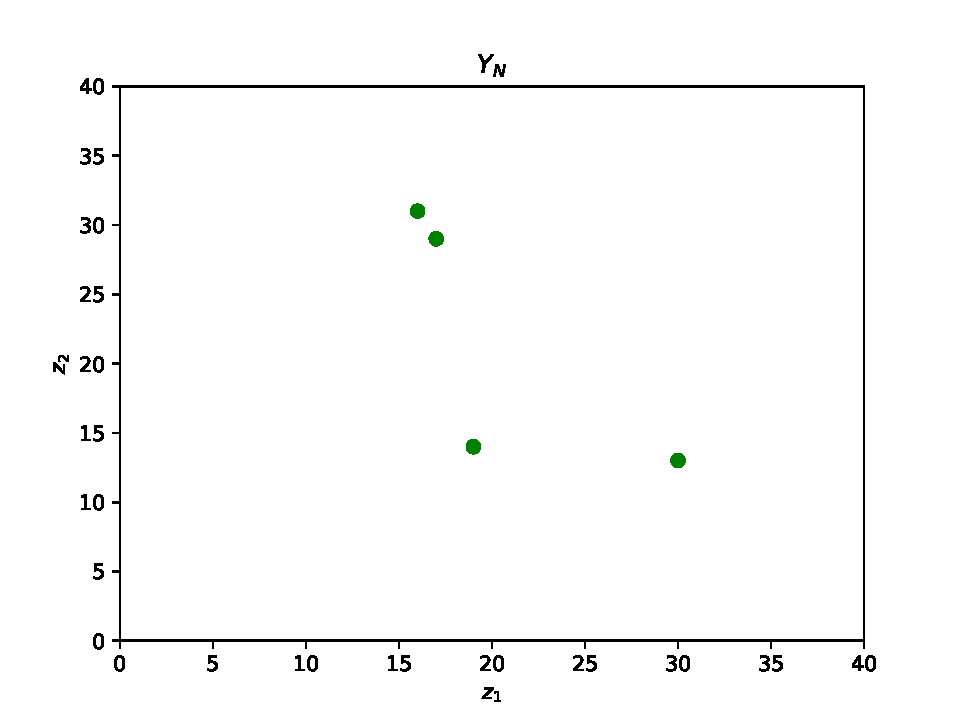
\includegraphics[scale=0.75]{figplot.pdf}
  \end{center}
%\break


\end{document}
